\subsection{Regular diffusion}
The idea of diffusion is to fix the known regions of the image and let them diffuse into the unknown regions. This can be done very efficiently by using a convolutional kernel. By iteratively convolving a kernel with the entire image and then restoring the known pixels we can obtain an inpainted image. This process is described in algorithm \ref{alg:diffusion}. The quality of the solution heavily depends on the kernel used. A variety of kernels can be used, two of which are displayed in figure \ref{fig:kernels}. To convolve a kernel with an image we have to refer to pixels outside of the border of the image. We replicate the borders of the image outwards so the kernel can properly refer to these values.

\begin{figure}
\begin{flalign*}
K_{\text{diamond}} &= \begin{bmatrix}0 & 0.25 & 0 \\ 0.25 & 0 & 0.25 \\ 0 & 0.25 & 0\end{bmatrix}\\
%K_{\text{gauss}} &= \begin{bmatrix}0.011 & 0.084 & 0.011\\0.084 & 0.620 & 0.084 \\0.011 & 0.084 & 0.011\end{bmatrix}\\
K_{\text{diag}} &= \begin{bmatrix}0.38 & 0.04 & 0.04 \\ 0.04 & 0 & 0.04 \\ 0.04 & 0.04 & 0.38\end{bmatrix}
\end{flalign*}
\caption{Kernels used for diffusion.}
\label{fig:kernels}
\end{figure}

\begin{algorithm}
	\KwIn{Image $I$, mask $M$, kernel $K$ and threshold $\epsilon$}
	\KwResult{Reconstructed image $I_{r}$}
	$K \leftarrow \frac{K}{\sum_i \sum_j K_{i,j}}$ (normalize $K$ to preserve energy)\; 
	$I_{prev} \leftarrow 0_{size(I)}$\;
	$I_{r} \leftarrow I$\;
	\While{$\|I_{r} - I_{prev} \|_{F} > \epsilon$}{
		$I_{prev} \leftarrow I_{r}$\;
		$I_{r} \leftarrow \text{convolve}(I_{r}, K)$\;
		$I_{r} \leftarrow I_{r} \circ \mathbf{1}_{M = 0} + I \circ \mathbf{1}_{M \neq 0}$ \;
	}
	\quad
\caption{Diffusion algorithm for inpainting. We denote element-wise multiplication with the $\circ$ operator. The $\mathbf{1}_{M=0}$ function represents a matrix with elements $(i,j)$ set to 1 when $M_{i,j}=0$ and 0 otherwise.}
\label{alg:diffusion}
\end{algorithm}
\begin{figure}
	\centering
	\begin{subfigure}[b]{0.4\textwidth}
		\centering
		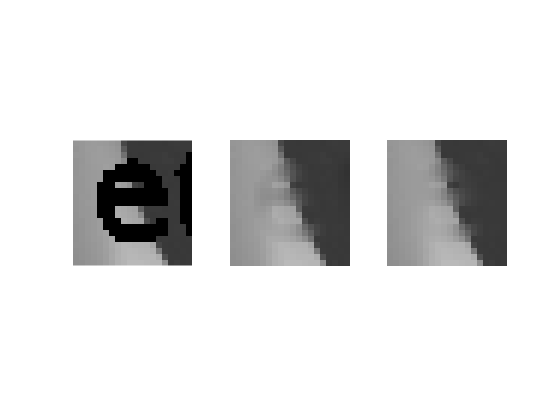
\includegraphics[clip, trim=0cm 5.2cm 0cm 4cm, width=0.85\textwidth]{figures/step-by-step-cross}
		\caption{Diamond kernel $K_{\text{diamond}}$}
		\label{fig:stepbystepcross}
	\end{subfigure}
	\begin{subfigure}[b]{0.4\textwidth}
		\centering
		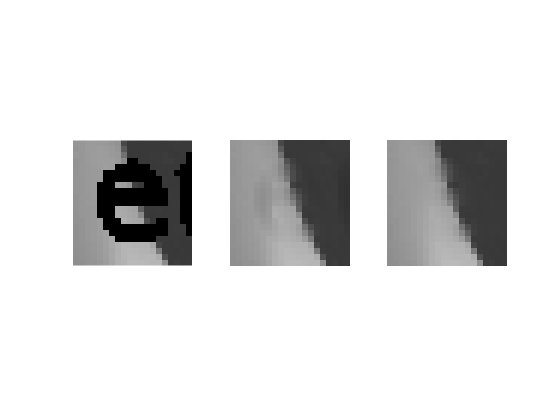
\includegraphics[clip, trim=0cm 5.2cm 0cm 4cm, width=0.85\textwidth]{figures/step-by-step-directional}
		\caption{Directional kernel $K_\theta$ for $\theta = 100\degree$.}
		\label{fig:stepbystepdir}
	\end{subfigure}
	\caption{Step-by-step illustration of the diffusion process with different kernels. Each step represent 20 iterations.}
\end{figure}